\documentclass[conference]{IEEEtran}
\usepackage[ruled,vlined]{algorithm2e}
\usepackage{amsmath}
\usepackage[english]{babel} %localisation
\usepackage{caption,subcaption} %supposedly incompatible with Springer and IOP, IEEETran and ACM SIG
\usepackage{cite} %nice citations, e.g. [1--5]
\usepackage{fixltx2e} %fix latex bugs
\usepackage{graphicx}
\PassOptionsToPackage{hyphens}{url}\usepackage{hyperref} %clickable URLS
\usepackage[htt]{hyphenat} %hyphenate \texttt
\usepackage{microtype} %makes text pretty; also condenses
\usepackage{multirow} %multiple rows in tables
\usepackage{siunitx,textcomp} %\SI{value}{unit}, \si{unit}; textcomp for microtype compatibility
%\usepackage [caption=false]{subfig} %if caption/subcaption not available
% \usepackage{tikz,pgfplots} %drawings and plots
\usepackage[siunitx]{circuitikz} %circuit figures
\usepackage[T1]{fontenc} %ensure proper hyphenation and treatment of math in sentences
\usepackage{booktabs}
\bibliographystyle{IEEEtran}

\usepackage{tikz}
\usepackage{verbatim}
\usepackage{listings}
\begin{document}
\lstset{defaultdialect=[x86]{Assembler}}

% paper title
% can use linebreaks \\ within to get better formatting as desired
\title{Reprogramming embedded systems using Return Oriented Programming}

% author names and affiliations
% use a multiple column layout for up to three different
% affiliations
\author{\IEEEauthorblockN{Sam Mitchell and Nathanael Weidler}
\IEEEauthorblockA{Deptartment of Electrical and Computer Engineering\\
Utah Stat University\\
Logan, Utah 84322\\
e-mail: samuel.alan.mitchell@gmail.com, NWeidler@gmail.com}
}

% make the title area
\maketitle


\begin{abstract}
%\boldmath
% Summarize project and results (executive summary).
% This paper describes the implementation of high-throughput password cracking devices. We consider architecture-aware implementations of password crackers on FPGA and X86 architectures. An analysis of speed and cost efficacy is included. 
This paper describes the theory and implementation of a return-oriented programming attack on a ARM-based device. The attack reprograms the device to execute our desired code upon reset. We describe the gadget searching process and the code injection method. 


% This paper considers the efficient computation of passwords. Multiple methods to increase hashing throughput are presented. It is shown that hardware implementation of a password cracker provides more throughput per unit dollar than a software implementation. Future research will address the efficacy of different architectures in password computation. 
\end{abstract}

\begin{IEEEkeywords}
Return Oriented Programming, Security, ARM, Harvard architecture.
\end{IEEEkeywords}

\section{Introduction}
	Single-purpose embedded devices such as voting machines or vehicle guidance controllers are generally considered to be secure machines. Previous work has shown that Return Oriented Programming (ROP) methods can be used to attack ARM-based devices \cite{checkoway2009can} \cite{Kunz}. % cite trevor, a few other papers. 

	ROP is a type of buffer-overflow attack that modifies the return address of the existing program, causing the program to execute existing code. In x86 architectures, ROP attacks generally jump into libc to control the behavior of the compromised program. An attack on an ARM-based device uses similar techniques --- manufacturer-provided peripheral driver libraries provide sufficient code-space to implement a devastating ROP attack.  

% Describe the problem and what you're doing to address it (i.e.\ building architecture-informed md5 password cracker for software and hardware; how password cracking operates).  

% \subsection{Related work}
% 	Previous work in efficient implementations of 
% What is needed to understand your optimisations and/or implementations.  Do you draw on existing techniques? If so, describe and cite them.

\subsection{Structure of paper}
	The organization is as follows: in Section \ref{sec::design}, the system design and modifications required to enable the ROP attack are presented. Section \ref{sec::asm} contains the desired program and code required to inject the program into the system without ROP. Gadgets to utilize in the ROP attack and the required sequence of execution are proposed in Section \ref{sec::gadget}. Section \ref{sec::results} describes the implementation methods, and Section \ref{res1} presents the results of the attack. Conclusions are discussed in Section \ref{sec::conclusion}. 

% Problems: 
% 	System design. Completed by Nathanael
% 	Exploitation. 

% Reporting requirements:
% 	Provide required assembly. 
% 	Gadgets (based on figure 16 of The Geometry of Innocent Flesh on the Bone)
% 	Injected stack. 
% 		Contents before and after overwriting the buffer. 
% 		Contents of flash before and after rewriting it. 
% 	Screenshot of executing the current code. 


\section{System design} \label{sec::design} % Nathanael
% write about the auth() function and the UART buffer check disable

As part of the preparation for the ROP implementation, we disabled some  optimizations in order to simplify the attack. The compiler flag -O0 was used instead of -O2, which made the assembly code more readable. Another compiler flag, --no\_protect\_stack, was used to remove canaries which alert the program when the stack is corrupted. The linker flag, --no\_remove, ensured that the included libraries were flashed to the board even if the code wasn't executed. This doubled our available code space, which allowed for more precise selection of gadgets. 

\section{Reprogramming method} \label{sec::asm} % Sam
The target of this project is to insert a program (see Figure \ref{fig::insert}) that will run at reset. The current main function is located at memory address 0x2aca. Executable memory must be reprogrammed through the Flash module (located at 0x400fd000). There are multiple methods to reprogram the code space at 0x2aca. 
	\begin{figure}[htbp]
		\lstset{language={[thumb]Assembler}} 
		\begin{lstlisting}
Start
	add R0, #0x1 	; 0xF1000001
	b Start		; 0xE7FC
		\end{lstlisting}
		\caption{The program to be inserted. }\label{fig::insert}
	\end{figure}

Flash memory can either be erased or programmed. Memory is erased (the bits are cleared to a value of 1) in 1kb chunks. Programming can only bring a bit from high to low (1 to 0). The most simple method to insert the program at main would be to overwrite existing code currently located at main. This method is only available if the desired command has 1s located in the same position as the existing command's 1s. See Figure \ref{fig::ham}. 
	\begin{figure}[htbp]
		\lstset{language={[thumb]Assembler}} 
		\begin{lstlisting}
Current instruction	0xE92D4FF0
Desired instruction	0xF1000001
		\end{lstlisting}
		\caption{Writing the desired instruction doesn't work because the current instruction bits would require 0 to 1 programming.  }\label{fig::ham}
	\end{figure}
The target program does not have convenient programming instructions, as can be seen in Figure \ref{fig::ham}. The memory at main must first be erased (written to 1s) then programmed. The procedures to erase, reprogram, and an alternate reprogramming sequence are located in Figures \ref{fig::erase}, \ref{fig::prog}, \ref{fig::alt_prog}, respectively. 
		\lstset{language=C} 
	\begin{figure}[htbp]
		\begin{lstlisting}
// base address
uint32_t * FLASH = (uint32_t *) 0x400FD000;
FLASH[0x0] = 0x4800; // address to erase
// clear the area 0x2800-0x2C00
// perform erase command
FLASH[0x8/4] = 0xA4420002; 
		\end{lstlisting}
		\caption{Erasing sequence. }\label{fig::erase}
	\end{figure}
	\begin{figure}[htbp]
		\begin{lstlisting}
// address to program
FLASH[0x0] = 0x4BA0; 
// add instruction
FLASH[0x4/4] = 0xF1000001; 
// perform write command
FLASH[0x8/4] = 0xA4420001; 

// address to program
FLASH[0x0] = 0x4BA4; 
// branch instruction
FLASH[0x4/4] = 0xE7FC0000; 
// perform write command
FLASH[0x8/4] = 0xA4420001; 
		\end{lstlisting}
		\caption{Reprogramming sequence. }\label{fig::prog}
	\end{figure}
	\begin{figure}[htbp]
		\begin{lstlisting}
// address to program
FLASH[0x0] = 0x4AE0; 
// add instruction
FLASH[0x120/4] = 0xF1000001;
// branch instruction
FLASH[0x124/4] = 0xE7FC0000;
// force enable write 
FLASH[0x30/4] = 0xFFFFFFFF;
// perform write command
FLASH[0x20/4] = 0xA4420001; 
		\end{lstlisting}
		\caption{Alternative reprogramming sequence.  }\label{fig::alt_prog}
	\end{figure}

Translating the rewrite procedure into assembly will require a load / move / pop instruction to populate registers, followed by a store command to write to memory. The load / move / pop command is discussed in Section \ref{sec::gadget}. 




\section{Gadgets} \label{sec::gadget} % not completed
The basic operation of ROP is performed by redirecting the locations jumped to via buffer overflow. This method does not actually insert any executable code onto the stack --- existing code is merely utilized in creative ways. Gadgets are the building blocks of ROP. Any gadget used in ROP must contain a return-like command. 

Because Thumb assembly does not contain any return commands, alternatives to this command must be used. Two such instructions are bx and pop \{pc\}. The bx / pop and the preceding lines of code are what constitute a gadget. Many gadgets exist, but careful selection can produce a turing-complete instruction set. 

The flash rewrite sequence contained in Figures \ref{fig::erase} and \ref{fig::alt_prog} requires two operations: load and store. Our search for gadgets resulted in two effective sets of instructions, located in Figure \ref{fig::gadget1}. 

	\begin{figure}[htbp]
		\lstset{language={[thumb]Assembler}} 
		\begin{lstlisting}
; Gadget A
str R0, [R4,#0x0]
pop {R4,PC}

; Gadget B
mov R0, R4
pop {R4-R6,PC}
		\end{lstlisting}
		\caption{Gadgets that provide the required load and store operations. }\label{fig::gadget1}
	\end{figure}
% Table generated by Excel2LaTeX from sheet 'Sheet1'
Gadget A: this gadget provides the ability to store data from R0 into the address specified at R4. It also causes the program to jump to the next instruction, while filling R4 with more data from the stack. This gadget is effective because R4 is constantly updated. 

Gadget B: this gadget transfers the data from R4 into R0. There were no gadgets that would load R0 directly, so this method was a sufficient substitute. The data from the stack is transferred from the stack to R4 during Gadget A, followed by Gadget B where the data is shuttled to R0 while R4 is repopulated. Finally, the data is stored into the desired location via Gadget A. 



% \section{ROP design}\label{sec::rop} % not completed
The design of the ROP was taken directly from the code in Figures \ref{fig::erase} and \ref{fig::alt_prog}. The gadgets in Figure \ref{fig::gadget1} were combined in a pipelined fashion in order to minimize operations. Our implementation was still rather bulky at 13 required returns. The number of returns could have been reduced by finding gadgets containing the STR2 command, which stores two words at an address. Table \ref{tab:gadgets} describes the order that the gadgets should be executed in order to rewrite the flash memory of the TM4C123GH6PM.

\begin{table}[htbp]
  \centering
  \caption{The required inputs and gadget sequence to execute the flash rewrite sequence in Figures \ref{fig::erase} and \ref{fig::alt_prog}. }
    \begin{tabular}{rrr}
    \toprule
    \multicolumn{1}{c}{Gadget} & \multicolumn{1}{c}{R4 input} & \multicolumn{1}{c}{Resulting code} \\
    \midrule
    \multicolumn{1}{l}{A} & \multicolumn{1}{l}{0x00004800} & \multicolumn{1}{l}{\textit{// Erase procedure}} \\
    \multicolumn{1}{l}{B} & \multicolumn{1}{l}{0x400FD000} & \multicolumn{1}{l}{uint32\_t * FLASH = (uint32\_t *) 0x400FD000;} \\
    \multicolumn{1}{l}{A} & \multicolumn{1}{l}{0xA4420002} & \multicolumn{1}{l}{FLASH[0x0] = 0x4800;} \\
    \multicolumn{1}{l}{B} & \multicolumn{1}{l}{0x400FD008} & \multicolumn{1}{l}{FLASH[0x8/4] = 0xA4420002;} \\
    \multicolumn{1}{l}{A} & \multicolumn{1}{l}{0x00004BD8} & \multicolumn{1}{l}{\textit{// Write procedure}} \\
    \multicolumn{1}{l}{B} & \multicolumn{1}{l}{0x400FD000} & \multicolumn{1}{l}{FLASH[0x0] = 0x4BD8;} \\
    \multicolumn{1}{l}{A} & \multicolumn{1}{l}{0xF1000001} & \multicolumn{1}{l}{FLASH[0x100/4] = 0xF1000001;} \\
    \multicolumn{1}{l}{B} & \multicolumn{1}{l}{0x400FD100} & \multicolumn{1}{l}{} \\
    \multicolumn{1}{l}{A} & \multicolumn{1}{l}{0xE7FC****} & \multicolumn{1}{l}{FLASH[0x104/4] = 0xE7FC****;} \\
    \multicolumn{1}{l}{B} & \multicolumn{1}{l}{0x400FD104} & \multicolumn{1}{l}{} \\
    \multicolumn{1}{l}{A} & \multicolumn{1}{l}{0xA4420001} & \multicolumn{1}{l}{FLASH[0x8/4] = 0xA4420001;} \\
    \multicolumn{1}{l}{B} & \multicolumn{1}{l}{0x400FD008} & \multicolumn{1}{l}{} \\
    \multicolumn{1}{l}{A} & \multicolumn{1}{l}{} & \multicolumn{1}{l}{\textit{// Return to 0x4BD8}} \\

    \bottomrule
    \end{tabular}%
  \label{tab:gadgets}%
\end{table}%


\section{Implementation}\label{sec::results} % not completed 
The ROP attack was first approached by determining the size and boundaries of the stack (see Figure \ref{fig::stack}). Once the boundaries were determined, we replaced the location which would be popped into the program counter (PC) with the address of Gadget A. Each successive call (shown in Table \ref{tab:gadgets}) was determined by overwriting the values to be placed into the R4 and PC registers.

The attack outlined in Table \ref{tab:gadgets} was performed and resulted in the desired functionality until the device was reset. Upon reset, the program would jump to a scatter function located in the previously erased region. This resulted in an interrupt which prevented the device from executing the program located at the address of main(). This was solved by inserting data falsification at the scatter function. 
% Author: Rasmus Pank Roulund

\usetikzlibrary{shapes,arrows,positioning}
\tikzstyle{block} = [draw, fill=white, rectangle, 
    minimum height=2em, minimum width=6em]
\tikzstyle{input} = [coordinate]
\tikzstyle{output} = [coordinate]
\tikzstyle{pinstyle} = [pin edge={to-,thin,black}]
\begin{figure}[htbp]

\begin{tikzpicture}[auto, node distance=2em,>=latex']
% \begin{scope}[node distance=3em and 20em]%Here we change it for everything inside this scope
  % \node [block,name=stack] {Stack};
  % \node [output, right= 2em of stack] (rstack) {};
  % \node [output, left= 2em of stack] (lstack) {};


  \node [block,below of=block] (uname) {Username};
  \node [block,below of =uname] (passd) {Password};

  \node [output, right= 2em of uname] (runame) {};
  \node [output, right= 2em of passd] (rpassd) {};
 
  \node [output, left= 2em of uname] (luname) {};
  \node [output, left= 2em of passd] (lpassd) {};



  \draw [->] (uname) -- (runame) -- (rpassd) -- (passd);
  % \draw [->] (stack) -- (lstack) -- (luname) -- (uname);

\end{tikzpicture}
\caption{The ROP attack construction. }
\label{fig::stack}
\end{figure}
% \begin{lstlisting}
% bottom of 
% memory    

% \end{lstlisting}

\section{Results}\label{res1}
The successful ROP attack works very well, as shown by the device executing the injected code in Figure \ref{fig::ex}.  The stack before the exploit is shown in Figure \ref{fig::st1}, with the corrupted stack shown in Figure \ref{fig::st2}. The flash memory is shown in the following states: original, erased, written, and rewritten in Figures \ref{fig::fl0}, \ref{fig::fl1}, \ref{fig::fl2}, \ref{fig::fl3}. 
\begin{figure}[htbp]
	\centering
	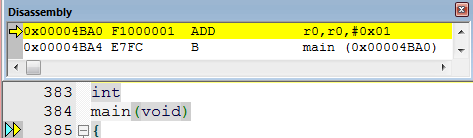
\includegraphics[width=0.8\textwidth]{ex.PNG}
	\caption{The device executing the injected code. }\label{fig::ex}
\end{figure}


\begin{figure}[p]
	\centering
	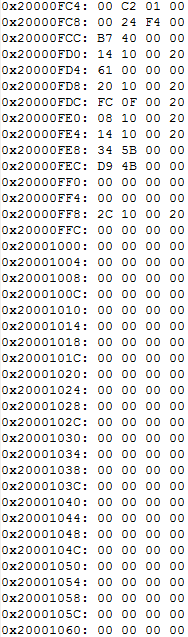
\includegraphics[\width=0.5\textwidth]{StackBefore1}
	\caption{The stack prior to any tampering. }\label{fig::st1}
\end{figure}
\begin{figure}[p]
	\centering
	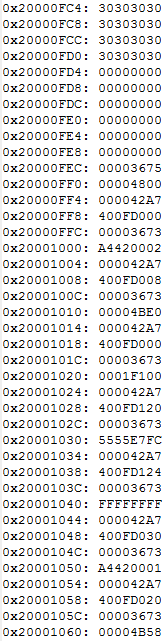
\includegraphics[\width=0.5 \textwidth]{stackAfter}
	\caption{The stack after corruption. }\label{fig::st2}
\end{figure}

\begin{figure}[p]
	\centering
	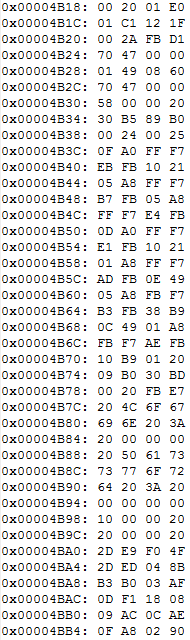
\includegraphics[\width=1in]{FlashBefore.PNG}
	\caption{The flash memory at main prior to any tampering. }\label{fig::fl0}
\end{figure}
\begin{figure}[p]
	\centering
	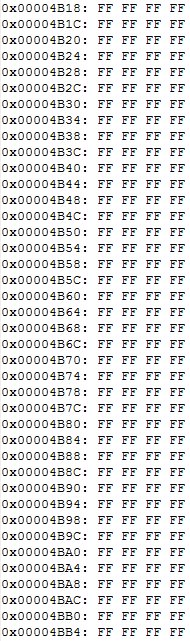
\includegraphics[\width=0.5\textwidth]{FlashAfterErase}
	\caption{The flash memory after the erase of main(). }\label{fig::fl1}
\end{figure}

\begin{figure}[p]
	\centering
	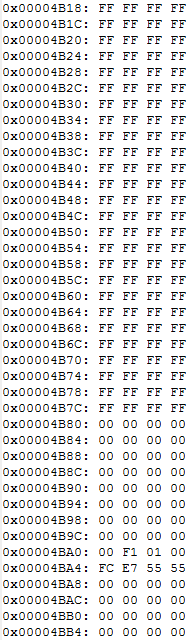
\includegraphics[\width=0.5\textwidth]{FlashAfterWrite1}
	\caption{The flash memory after the write to main(). }\label{fig::fl2}
\end{figure}

\begin{figure}[p]
	\centering
	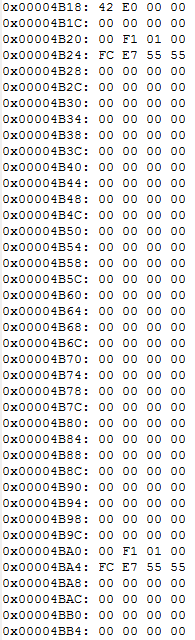
\includegraphics[\width=0.5\textwidth]{FlashAfterWrite2}
	\caption{The flash memory after the write to the scatter function. }\label{fig::fl3}
\end{figure}


\section{Conclusion}\label{sec::conclusion} 


% Summarize results and lessons learned.
	% This paper considers the efficient computation of passwords. Multiple methods to increase hashing throughput are presented. It is shown that hardware implementation of a password cracker provides more throughput per unit dollar than a software implementation. Future research will address the efficacy of different architectures in password computation. 
	This paper demonstrates an ROP attack on a Harvard-architecture device. It is shown that it is possible to insert a program that will return to execution after restart, while the device is still running. Future research will address the attack of the device without limitations imposed in Section \ref{sec::design}.
\bibliography{report}
% that's all folks




\end{document}